\chapter{Diseño}
\label{chap:diseño}

\lettrine{E}n este capítulo se tratará el diseño del sistema deliberativo desarrollado en este trabajo, cuyo objetivo principal es conseguir que el robot seleccione de manera autónoma las 
acciones a ejecutar en función de su objetivo y del conocimiento obtenido del entorno. El sistema se basa en la combinación de dos modelos aprendidos de forma independiente: el modelo de 
mundo, que permite predecir el estado siguiente tras realizar una accion, y el modelo de utilidad, que evalúa estos estados en función de lo deseables que son para cumplir cierto objetivo.


\section{Arquitectura del sistema}

La arquitectura del sistema deliberativo se estructura en 4 partes principales que se ejecutan en bucle hasta que el robot consigue alcanzar su meta:

\begin{itemize}
    \item Primero se obtienen las observaciones del estado actual (\(Obs_T\)) del robot y del objetivo.
    \item A continuación, se utiliza el modelo de mundo (WM) para predecir las observaciones del estado siguiente (\(Obs_{T+1}\)) para cada una de las acciones disponibles.
    \item Tras esto, se evalúa la utilidad (U) de cada uno de estos estados con el modelo de utilidad (UM).
    \item Finalmente, se ejecuta la acción con mayor utilidad en el robot.
\end{itemize}

La figura \ref{fig:esq_diseño} muestra un esquema sencillo de la estructura del sistema.

\begin{figure}[hp!]
  \centering
  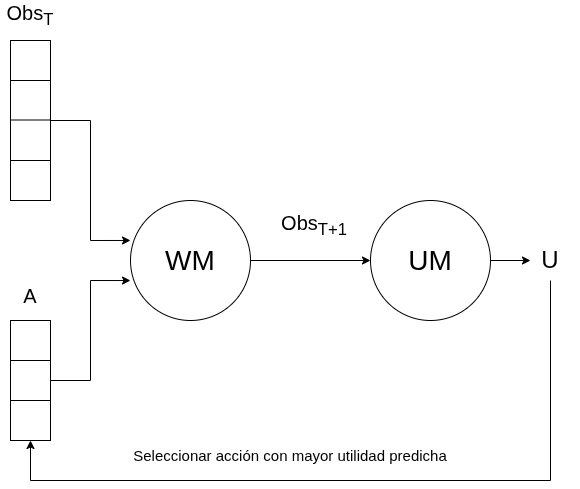
\includegraphics[width=0.75\textwidth]{imaxes/EsquemaDiseño.png}
  \caption{Estructura del sistema.}
  \label{fig:esq_diseño}
\end{figure}
